
\FloatBarrier
\section{Коливальна система з гістерезисом в силі, що повертає} % {{{1 _VGLASS_
\label{atu:sect:vglass}

\LinkRef{
  vglass: ITMM-2013
}

\subsection{Визначення системи та аналіз її динаміки} % {{{2 vglass_task

Коливальні системи з різними видами нелінійних залежностей
як в силі, що повертає, так і у члені при першій похідній,
часто розглядаються як потенційні кандидати в хаотичні
системи. Особливий інтерес представляють системи, нелінійні
компоненти яких відображають реальні елементи систем
управління~\cite{atu_st85,atu_ISDMCI2013,atu_asau20}. Одним з таких істотно
нелінійних елементів є гістерезис~\cite{sys_hyst, in_theory_mech_vibro,ivanov_alg_id_dyn_hyst, andronn_id_ns_hyst, mai_iss_dyn_isp}.
Розглянемо спочатку нестійку систему, яка стабілізується релейно-пропорційним стабілізуючим
впливом. Така система стабілізації активується при заданому
відхиленні величини, що спостерігається, а вимикається при
меншому. Така неоднозначність в поведінці систем стабілізації
призводить до різноманітних коливальних явищ поблизу
точки стабілізації, а всі спроби лінеаризації розглянутих
нелінійностей, в даному випадку, призводять до принципових
помилок в моделюванні.

Наявність точки нестійкої рівноваги, що вимагає стабілізуючого
впливу в більшому масштабі, явною, а часто і прихованої
нелінійності елементів системи, апріорна параметрична
невизначеність зовнішніх впливів --- все це створює передумови
для появи у систем складної коливальної динаміки, в тому числі
і хаотичної. Розглянемо рівняння, що задає динаміку цієї системи:
%
\begin{equation}
  \ddot{x} + c_o \dot{x} + r( x, \ldots ) = u(t),
  \label{atu:eq:vglass}
\end{equation}
%
де
$x(t)$ --- координата (вихідний сигнал),
$c_0$ --- безрозмірний коефіцієнт демпфірування,
$u(t) = U_{in} \sin (\omega_{in} t) $ --- зовнішня сила,
$r(x, \ldots) $ --- сила, що повертає, яка включає лінійну складову ($ax$,$ a <0 $),
що зумовлює нестійкість при малих
відхиленнях, і гістерезисну компоненту, яка задається
алгоритмічно. Характерний вид сили, що повертає, наведено на
рис.~\ref{atu:f:vg_rf}.

\begin{figure}[htb!]
\centerline{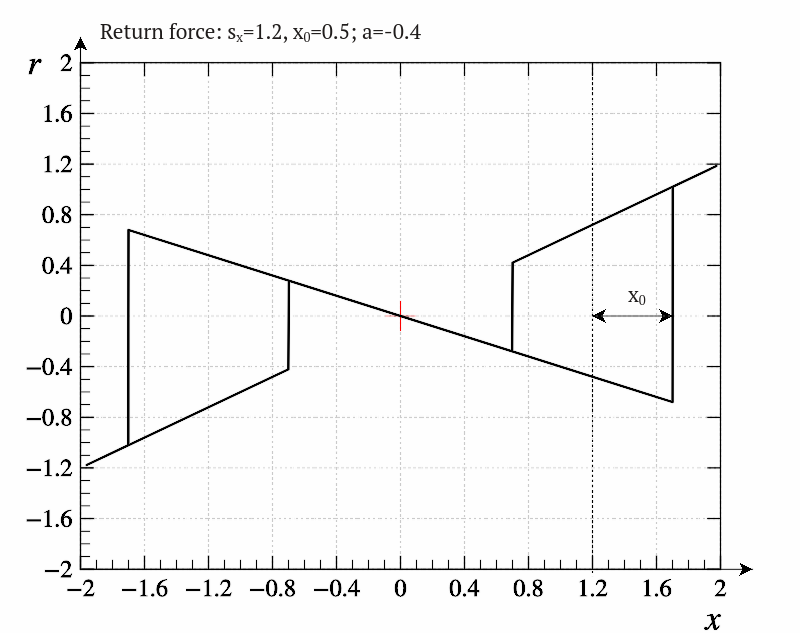
\includegraphics[width=0.5\textwidth]{p/cha/vg/vg_rf-p_rf.png} }
\caption{Гістерезисна сила, що повертає}
\label{atu:f:vg_rf}
\end{figure}

Параметрами цієї залежності, крім уже згаданого коефіцієнта
$a$, є
$s_x$ --- центральна точка включення і виключення стабілізуючого
впливу,
$x_0$ --- половина ширини гістерезису. Ширина петлі гістерезису
для даної системи визначає енергію, яку отримує система від
системи стабілізації в процесі роботи. Саме це величина і буде
ідентифікованим параметром.


На відміну від системи Дуффінга, розглянута система має власну
динаміку при відсутності впливу, що збурює. При малих значеннях
$x_0$ відбуваються нелінійні, але досить прості коливання по
одну сторону від точки
$x = 0$~(рис.~\ref{atu:f:vglass_phase_f_u00}), причому сторона визначається
початковими умовами. Спектр коливань досить бідний.

\begin{figure}[htb!]
  \PicDouble{p/cha/vg/vg_0-p_phe_0x00_0x70_0x12.png}{p/cha/vg/vg_fft-p_f_0x00_0x70_0x12.png}
  \caption{Розширений фазовий портрет~(a) і спектр~(b) системи (\ref{atu:eq:vglass}) при $ U_{in} = 0 $ і $ x_0 = 0.12 $}
\label{atu:f:vglass_phase_f_u00}
\end{figure}

При зростанні параметра
$x_0$ динаміка системи стає складнішою (рис.~\ref{atu:f:vglass_phase_f_u01}),
однак спектр системи залишається простим лінійчатим. Така
поведінка зберігається аж до природного обмеження
$ x_o <s_x $, при цьому фазовий портрет наближається до кола.

\begin{figure}[htb!]
  \PicDouble{p/cha/vg/vg_0-p_phe_0x00_0x70_0x15.png}{p/cha/vg/vg_fft-p_f_0x00_0x70_0x15.png}
  \caption{Розширений фазовий портрет~(a) і спектр(b) системи (\ref{atu:eq:vglass}) при $ U_{in} = 0 $ і $ x_0 = 0.15 $}
\label{atu:f:vglass_phase_f_u01}
\end{figure}

При наявності ненульового зовнішнього впливу
$u(t)$ картина помітно ускладнюється. Спостерігаються такі
значення параметра
$x_0$, при яких спостерігається складний аттрактор, характерний
для хаотичної динаміки~(рис.~\ref{atu:f:vglass_phase_f_u10}) і ділянки
суцільного спектра.

\begin{figure}[htb!]
  \PicDouble{p/cha/vg/vg_0-p_phe_0x20_0x70_0x05.png}{p/cha/vg/vg_fft-p_f_0x20_0x70_0x05.png}
  \caption{Розширений фазовий портрет~(a) і спектр~(b) системи (\ref{atu:eq:vglass}) при $ U_{in} = 0.2 $ і $ x_0 = 0.05 $}
\label{atu:f:vglass_phase_f_u10}
\end{figure}

Загальною властивістю цієї системи і системи Дуффінга є те, що
ділянка суцільного спектра примикає до точки нульової частоти,
що ускладнює процес усереднення критерію.

Також спостерігаються такі діапазони
$ x_0 $, в яких спостерігаються регулярні коливання
(рис.~\ref{atu:f:vglass_phase_f_u11}).

\begin{figure}[htb!]
  \PicDouble{p/cha/vg/vg_0-p_phe_0x20_0x70_0x40.png}{p/cha/vg/vg_fft-p_f_0x20_0x70_0x40.png}
  \caption{Розширений фазовий портрет~(a) і спектр~(b) системи (\ref{atu:eq:vglass}) при $ U_{in} = 0.2 $ і $ x_0 = 0.40 $}
\label{atu:f:vglass_phase_f_u11}
\end{figure}

Крім регулярних коливань, спостерігаються режими
складно-періодичної динаміки, з складним аттрактором і
спектром, в якому спостерігається ряд близько розташованих
піків (рис.~\ref{atu:f:vglass_phase_f_u12}).

\begin{figure}[htb!]
  \PicDouble{p/cha/vg/vg_0-p_phe_0x20_0x70_0x70.png}{p/cha/vg/vg_fft-p_f_0x20_0x70_0x70.png}
  \caption{Розширений фазовий портрет~(a) і спектр~(b) системи (\ref{atu:eq:vglass}) при $ U_{in} = 0.2 $ і $ x_0 = 0.70 $}
\label{atu:f:vglass_phase_f_u12}
\end{figure}

Таку поведінка складно, а в разі нестаціонарного значення
параметра може бути і неможливо відрізнити від хаотичної
поведінки.

Таким чином, так як система в робочому діапазоні параметра
$x_0$ демонструє різні види динамік, в тому числі хаотичну,
то для ідентифікації має сенс розглянути набір методів, що
розглядаються в даній роботі.

% }}}2

\subsection{Аналіз і вибір критерію} % {{{2

При синтезі критерію для нелінійної коливальної системи, якщо
немає можливості використовувати будь-якої явний і очевидний
критерій, в першу чергу слід розглянути критерії виду
$q_{x^2}$,
$q_{rx}$ і
$q_T$. Так як гістерезисна сила, що повертає, не дає можливості
використовувати аналітичний підхід, то розглянемо залежності
$q_{rx} $ і
$q_T$ (рис.~\ref{atu:f:vglass_q}), отримані шляхом чисельного моделювання.

\begin{figure}[htb!]
\begin{center}
  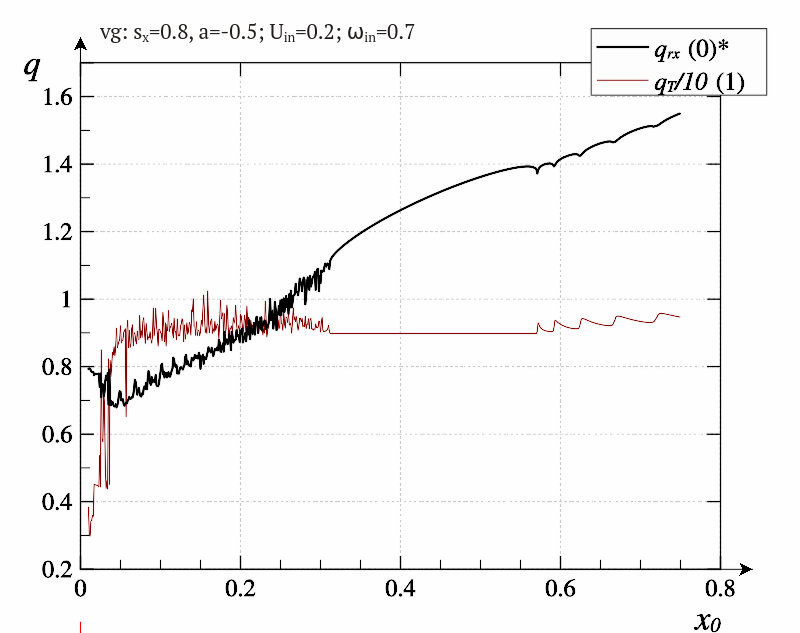
\includegraphics[width=0.49\textwidth]{p/cha/vg/vg_q1-p_q.png}
\end{center}
  \caption{Залежності $q_{rx}(x_0)$ і $q_T(x_0)$ для системи (\ref{atu:eq:vglass})}
\label{atu:f:vglass_q}
\end{figure}

Аналіз залежностей дозволяє зробити висновок про те, що критерій
$q_T$ непридатний для ідентифікації параметра
$x_0$ даної системи, з огляду на те, що залежність від параметра,
якщо не брати до уваги коливання, практично відсутня.

Застосування критерію
$q_{rx} $ досить суперечливо. З одного боку, в цілому
спостерігається близька до лінійної залежність, що знижує
вимоги до тонкої настройки системи ідентифікації. З іншого
боку, на тих ділянках, де спостерігаються переходи від
складно-періодичних коливань до хаотичних, монотонність
залежності порушується. Однак, амплітуда цих збурень невелика,
що дає можливість побудови працездатної системи ідентифікації,
але з істотними обмеженнями на досяжну точність. Таким чином,
на брак кращого, будемо використовувати цей критерій.


% }}}2

\subsection{Тестова задача ідентифікації} % {{{2

Для ідентифікації параметра
$x_0$ коливальні системи з гістерезисної силою, що повертає, була
використана група методів ``ql3rlWvnAAW''. Використання критерію
$q_{rx}$ для даної системи, з урахуванням наявності ділянок
відсутності монотонності вимагає окремої перевірки
працездатності, так як використовуваний раніше підхід
з повільно змінюючимся параметром (\ref{atu:eq:po_t_ramp}) не дозволяє
відокремити похибку, пов'язану з встановленням режиму системи
ідентифікації від похибки, викликаної не цілком адекватним
критерієм.

Для визначення похибки ідентифікації без впливу перехідних
процесів, була проведена серія обчислювальних експериментів.
На кожному з них значення параметра
$x_0$ було фіксовано. Діапазон зміни цього параметра було обрано
$[0,2; 0.6] $. Попередньо була зроблена перевірка, що за повний час
ідентифікації
$T = 1000 $ всі перехідні процеси дійсно завершилися. Залежність
отриманої похибки ідентифікації від значення параметра
$x_0 $ для різних способів оцінювання
$p_\mathrm{id} $ представлена на рис.~\ref{atu:f:vg_id_scan}.

\begin{figure}[htb!]
\begin{center}
  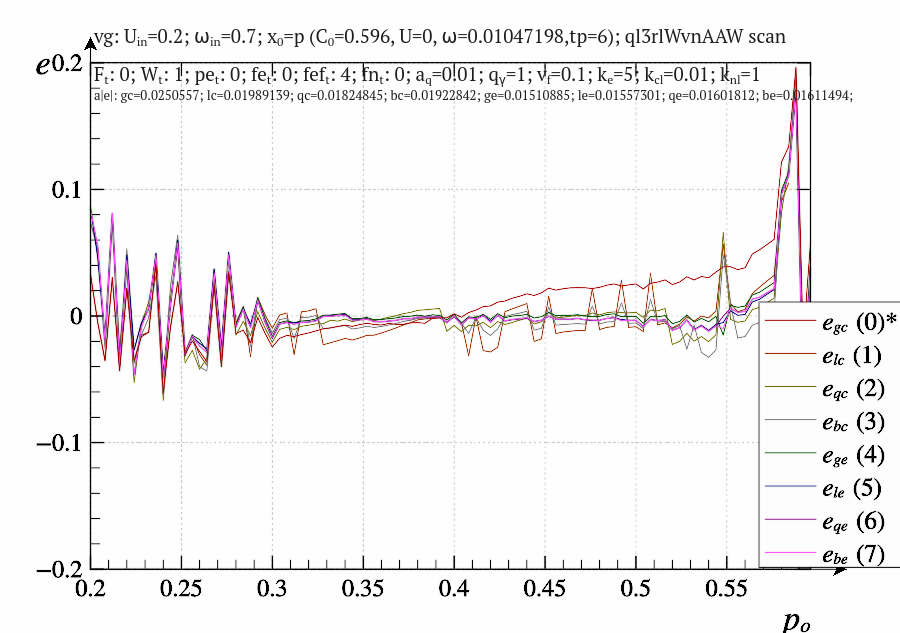
\includegraphics[width=0.60\textwidth]{p/cha/vg/vg_id-p_p_e_ql3rlWvnAAW_scan.png}
\end{center}
\caption{Залежності $e(x_0) $ для коливальної системи з гістерезисною силою, що повертає }
\label{atu:f:vg_id_scan}
\end{figure}

Аналіз отриманих залежностей показує, що в тих областях, де
порушується монотонність критерію, похибка ідентифікації
значно зростає. Однак, рівень цієї похибки, за винятком однієї
вузької області, не перевищує вихідної відстані між агентами,
що дозволяє зробити висновок, що система ідентифікації
виявляється працездатною і в цьому несприятливому випадку.

Розглянемо динаміку агентів і ідентифікованого значення
(рис.~\ref{atu:f:vg_id_sign}) в разі істотно нестаціонарного параметра. При
цьому динаміка величини
$x_0 (t) $ задається (\ref{atu:eq:po_t_sign}),
$p_0 = 0.4$,
$U_p = 0.14$,
$\omega_p = \pi/300 $.

\begin{figure}[htb!]
  \PicDouble{p/cha/vg/vg_id-p_t_pi_ql3rlWvnAAW_sign.png}{p/cha/vg/vg_id-p_t_p_ql3rlWvnAAW_sign.png}
  \caption{Динаміка агентів~(a) і ідентифікованого значення~(b) для системи коливальні системи з гістерезисною силою, що повертає, за умови (\ref{atu:eq:po_t_sign})}
\label{atu:f:vg_id_sign}
\end{figure}

У розглянутих умовах на величину похибки ідентифікації
негативно впливають два фактори: те, що ділянка суцільного спектра примикає до нульової частоті,
а також відсутність монотонності
критерію в області мінімального значення параметра. Це
призводить до значних похибок в процесі ідентифікації, при
збереженні працездатності методу.


На рис.~\ref{atu:f:vg_id_sin} наведені аналогічні залежності, але за
умови~(\ref{atu:eq:po_t_sign}).

\begin{figure}[htb!]
  \PicDouble{p/cha/vg/vg_id-p_t_pi_ql3rlWvnAAW_sin.png}{p/cha/vg/vg_id-p_t_p_ql3rlWvnAAW_sin.png}
  \caption{Динаміка агентів~(a) і ідентифікованого значення~(b) для системи коливальні системи з гістерезисною силою, що повертає, за умови (\ref{atu:eq:po_t_sin})}
\label{atu:f:vg_id_sin}
\end{figure}

Більш плавна зміна параметра, як і в попередніх випадках,
призводить до зменшення похибки ідентифікації. Однак,
вид критерію не дозволяє отримати досить малу похибку
ідентифікації.



% }}}2

\subsection{Вплив параметрів системи ідентифікації на похибку ідентифікації} % {{{2

Вплив параметра
$ a_q $ на похибку ідентифікації для коливальної системи з
гістерезисною силою, що повертає, має вигляд, типовий для систем зі
спектром, що прилягає до нульової частоті~(рис.~\ref{atu:f:vg_e_a_q}). Немає
явно вираженого мінімуму, що свідчить про обмеженість
фільтруючих властивостей підходу до усереднення критерію.

\begin{figure}[htb!]
  \PicDouble{p/cha/vg/vg_id-p_a_q_sign.png}{p/cha/vg/vg_id-p_a_q_sin.png}
  \caption{Залежності $\bar{e}(a_q) $ для коливальної системи з гістерезисною силою, що повертає за умов (\ref{atu:eq:po_t_sign})~(a) і (\ref{atu:eq:po_t_sin})~(b)}
\label{atu:f:vg_e_a_q}
\end{figure}

На тлі відносно високої похибки ідентифікації, яка визначається
властивостями критерію, залежність від масштабу функції якості
(рис.~\ref{atu:f:vg_e_q_gamma}) досить мала, якщо, звичайно, параметр
$q_\gamma $ системи ідентифікації знаходиться в розумних межах.

\begin{figure}[htb!]
  \PicDouble{p/cha/vg/vg_id-p_q_gamma_sign.png}{p/cha/vg/vg_id-p_q_gamma_sin.png}
  \caption{Залежності $\bar{e}(q_\gamma)$ для коливальної системи з гістерезисною силою, що повертає за умов (\ref{atu:eq:po_t_sign})~(a) і (\ref{atu:eq:po_t_sin})~(b)}
\label{atu:f:vg_e_q_gamma}
\end{figure}

Властивості критерію
$q_{rx}$ для даної системи також обумовлюють слабку залежність
похибки ідентифікації від параметра
$v_f$ (рис.~\ref{atu:f:vg_e_v_f}).
Для швидко мінливого параметра переміщення агентів може бути не доцільним.

\begin{figure}[htb!]
  \PicDouble{p/cha/vg/vg_id-p_v_f_sign.png}{p/cha/vg/vg_id-p_v_f_sin.png}
  \caption{Залежності $\bar{e}(v_f)$ для коливальної системи з гістерезисною силою, що повертає}
\label{atu:f:vg_e_v_f}
\end{figure}

Абсолютно аналогічна картина спостерігається для параметра
$k_e$~(рис.~\ref{atu:f:vg_e_k_e}).

\begin{figure}[htb!]
  \PicDouble{p/cha/vg/vg_id-p_k_e_sign.png}{p/cha/vg/vg_id-p_k_e_sin.png}
  \caption{Залежності $\bar{e}(k_e)$ для коливальної системи з гістерезисною силою, що повертає за умов (\ref{atu:eq:po_t_sign})~(a) і (\ref{atu:eq:po_t_sin})~(b)}
\label{atu:f:vg_e_k_e}
\end{figure}

Вид залежності
$\bar{e} (k_{nl}) $ для даної системи має певні
відмінності~(рис.~\ref{atu:f:vg_e_k_nl}). Слабо виражений, але все ж
помітний мінімум спостерігається при значеннях
$k_{nl}$, який практично збігається з використовуваним значенням
$k_e$. Це можна пояснити тим, що більша квазірівноважна відстань
між агентами дозволяє в якійсь мірі нівелювати збурення
критерію невеликої амплітуди.

\begin{figure}[htb!]
  \PicDouble{p/cha/vg/vg_id-p_k_nl_sign.png}{p/cha/vg/vg_id-p_k_nl_sin.png}
  \caption{Залежності $\bar{e}(k_{nl})$ для коливальної системи з гістерезисною силою, що повертає за умов (\ref{atu:eq:po_t_sign})~(a) і (\ref{atu:eq:po_t_sin})~(b)}
\label{atu:f:vg_e_k_nl}
\end{figure}

Використання неоднозначного критерію, в сукупності з
обмеженнями на переміщення агентів робить залежність
$ \bar{e} (k_{cl}) $ (рис.~\ref{atu:f:vdp_e_k_cl}) практично відсутньою.


\begin{figure}[htb!]
  \PicDouble{p/cha/vg/vg_id-p_k_cl_sign.png}{p/cha/vg/vg_id-p_k_cl_sin.png}
  \caption{Залежності $\bar{e}(k_{cl})$ для коливальної системи з гістерезисною силою, що повертає за умов (\ref{atu:eq:po_t_sign})~(a) і (\ref{atu:eq:po_t_sin})~(b)}
\label{atu:f:vg_e_k_cl}
\end{figure}



% }}}2


\subsection{Висновки} % {{{2

Результати моделювання як динаміки системи~(\ref{atu:eq:vglass}) так і
процесів ідентифікації її параметра
$ x_0 $ дозволяють зробити наступні висновки:

\begin{itemize}

  \item
    Коливальна система з гістерезисною силою, що повертає,
    під впливом
    зовнішньої гармонійного збурення може демонструвати різні
    види динамік, в тому числі складно-періодичну і хаотичну.


  \item
    Критерій
    $ q_{rx} $ підходить для ідентифікації параметра ``$x_0$'' коливальної
    системи з гістерезисною силою, що повертає, але характеризується порушеннями
    монотонності, що істотно збільшує похибку ідентифікації.

  \item
    Наявність суцільного спектра системи, що примикає до нульової
    частоті, ускладнює завдання коректного усереднення критерію.

  \item
    Група методів ql3rlWvnAAW показала свою хорошу працездатність навіть
    в умовах використання критерію з обмеженими можливостями.


\end{itemize}
% }}}2

% }}}1

% vim: fdm=marker foldlevel=1 foldignore="%#" fdc=4 ft=tex
